\RequirePackage{fix-cm} % fix some latex issues see: http://texdoc.net/texmf-dist/doc/latex/base/fixltx2e.pdf
\documentclass[ twoside,openright,titlepage,numbers=noenddot,headinclude,%1headlines,% letterpaper a4paper
                footinclude=true,cleardoublepage=empty,abstractoff, % <--- obsolete, remove (todo)
                BCOR=5mm,paper=a4,fontsize=11pt,%11pt,a4paper,%
                ngerman,american,%
                ]{scrreprt}
% ****************************************************************************************************
% classicthesis-config.tex 
% formerly known as loadpackages.sty, classicthesis-ldpkg.sty, and classicthesis-preamble.sty 
% Use it at the beginning of your ClassicThesis.tex, or as a LaTeX Preamble 
% in your ClassicThesis.{tex,lyx} with % ****************************************************************************************************
% classicthesis-config.tex 
% formerly known as loadpackages.sty, classicthesis-ldpkg.sty, and classicthesis-preamble.sty 
% Use it at the beginning of your ClassicThesis.tex, or as a LaTeX Preamble 
% in your ClassicThesis.{tex,lyx} with % ****************************************************************************************************
% classicthesis-config.tex 
% formerly known as loadpackages.sty, classicthesis-ldpkg.sty, and classicthesis-preamble.sty 
% Use it at the beginning of your ClassicThesis.tex, or as a LaTeX Preamble 
% in your ClassicThesis.{tex,lyx} with \input{classicthesis-config}
% ****************************************************************************************************  
% If you like the classicthesis, then I would appreciate a postcard. 
% My address can be found in the file ClassicThesis.pdf. A collection 
% of the postcards I received so far is available online at 
% http://postcards.miede.de
% ****************************************************************************************************


% ****************************************************************************************************
% 0. Set the encoding of your files. UTF-8 is the only sensible encoding nowadays. If you can't read
% äöüßáéçèê∂åëæƒÏ€ then change the encoding setting in your editor, not the line below. If your editor
% does not support utf8 use another editor!
% ****************************************************************************************************
\PassOptionsToPackage{usenames,dvipsnames}{xcolor}%needed because several packages include xcolor
\PassOptionsToPackage{utf8}{inputenc}
\usepackage{inputenc}
        
% ****************************************************************************************************
% 1. Configure classicthesis for your needs here, e.g., remove "drafting" below 
% in order to deactivate the time-stamp on the pages
% ****************************************************************************************************

% \PassOptionsToPackage{eulerchapternumbers,listings,%drafting,%
%					 pdfspacing,%floatperchapter,%linedheaders,%
%					 subfig,beramono,eulermath,parts}{arsclassica}

\PassOptionsToPackage{
  drafting=false,    % print version information on the bottom of the pages
  tocaligned=false, % the left column of the toc will be aligned (no indentation)
  dottedtoc=false,  % page numbers in ToC flushed right
  eulerchapternumbers=true, % use AMS Euler for chapter font (otherwise Palatino)
  linedheaders=false,       % chaper headers will have line above and beneath
  floatperchapter=true,     % numbering per chapter for all floats (i.e., Figure 1.1)
  minionprospacing=true,
  eulermath=true,  % use awesome Euler fonts for mathematical formulae (only with pdfLaTeX)
  beramono=true,    % toggle a nice monospaced font (w/ bold)
  palatino=true,    % deactivate standard font for loading another one, see the last section at the end of this file for suggestions
  style=arsclassica % classicthesis, arsclassica
}{classicthesis}


% ********************************************************************
% Available options for classicthesis.sty 
% (see ClassicThesis.pdf for more information):
% drafting
% parts nochapters linedheaders
% eulerchapternumbers beramono eulermath pdfspacing minionprospacing
% tocaligned dottedtoc manychapters
% listings floatperchapter subfig
% ********************************************************************

\usepackage{url}
\usepackage{nameref}
\usepackage{epigraph} %used for neat epigraphs at begging of chapters
\usepackage{verse}
\usepackage{datetime} %needed to add the date just below
\usepackage{pdflscape} %used to rotate pages with wide tables
\usepackage{rotating} %used to rotate wide figures
\usepackage{siunitx} %used for nice number formatting
\usepackage{pgf} % needed for arrays among other things
% ****************************************************************************************************
% 2. Personal data and user ad-hoc commands
% ****************************************************************************************************

\renewcommand{\epigraphsize}{\scriptsize}

\def\authors{
  {Student No 1/Student ID 1},
  {Student No 2/Student ID 2},
  {Student No 3/Student ID 3},
  {Student No 4/Student ID 4}}
\def\myTitle{Experimental CS Thesis Title\xspace}
\def\mySubtitle{A Guide for Content \& Style\xspace}
\def\myDegree{Master's Thesis\xspace}
\def\myShortNames{Student 1, 2, 3 \& 4\xspace}
\def\myGroup{My Group}
%\newcommand{\myStudentId}{20051234\xspace}
%\newcommand{\myNameToo}{Put Other Student Name Here\xspace}
%\newcommand{\myStudentIdToo}{20051235\xspace}
\def\myProf{Niels Olof Bouvin\xspace}
\def\myOtherProf{Put name here\xspace}
\def\mySupervisor{Put name here\xspace}
\def\myFaculty{Faculty of Natural Sciences\xspace}
\def\myDepartment{Department of Computer Science\xspace}
\def\myUni{Aarhus University\xspace}
\def\myLocation{Aarhus\xspace}
\def\myTime{\monthname\ \the\year\xspace}
\def\myVersion{\xspace}


% ********************************************************************
% Setup, finetuning, and useful commands
% ********************************************************************
\newcounter{dummy} % necessary for correct hyperlinks (to index, bib, etc.)
\newlength{\abcd} % for ab..z string length calculation
\providecommand{\mLyX}{L\kern-.1667em\lower.25em\hbox{Y}\kern-.125emX\@}
\providecommand{\mBibTeX}{\textsc{Bib}\negthinspace\TeX\@}
% ****************************************************************************************************


% ****************************************************************************************************
% 3. Loading some handy packages
% ****************************************************************************************************
% ******************************************************************** 
% Packages with options that might require adjustments
% ******************************************************************** 
%\PassOptionsToPackage{ngerman,american}{babel}   % change this to your language(s)
% Spanish languages need extra options in order to work with this template
%\PassOptionsToPackage{spanish,es-lcroman}{babel}
\usepackage[american]{babel}                  
\usepackage{microtype}
\usepackage{csquotes}
\usepackage{ragged2e}
% \usepackage[usenames,dvipsnames]{xcolor}
\usepackage{xcolor}
\usepackage{pgf-umlsd}
\usepackage{pgfplots}
\usepackage{pgfplotstable}
% recommended:
\usepackage{booktabs}
\usepackage{array}
\usepackage{colortbl}
% \usepackage{color}
\definecolor{aublue}{HTML}{193b77} % the dark blue colour used by AU

% Modify the biblabel format to use aublue for the source attribution
\renewcommand{\mkcitation}[1]{\xspace\textcolor{aublue}{[#1]}}




%\usepackage[square,numbers,sort&compress]{natbib}
%\bibliographystyle{abbrvnat}

\PassOptionsToPackage{%
   %backend=biber, %instead of bibtex
	backend=bibtex8,bibencoding=ascii,%
	language=auto,%
	style=numeric-comp,%
   %style=authoryear-comp, % Author 1999, 2010
   %bibstyle=authoryear,dashed=false, % dashed: substitute rep. author with ---
   sorting=nyt, % name, year, title
   maxbibnames=10, % default: 3, et al.
   %backref=true,%
   natbib=true % natbib compatibility mode (\citep and \citet still work)
}{biblatex}
\usepackage{biblatex}

\PassOptionsToPackage{fleqn}{amsmath}       % math environments and more by the AMS 
\usepackage{amsmath}
%
% ******************************************************************** 
% General useful packages
% ******************************************************************** 
\PassOptionsToPackage{T1}{fontenc} % T2A for cyrillics
\usepackage{fontenc}     
\usepackage{textcomp} % fix warning with missing font shapes
\usepackage{scrhack} % fix warnings when using KOMA with listings package          
\usepackage{xspace} % to get the spacing after macros right  
\newcommand{\eg}{e.g.,\xspace}
\newcommand{\Eg}{E.g.,\xspace}
\newcommand{\etal}{et~al.\xspace}
\newcommand{\etc}{etc.\@\xspace}
\newcommand{\ie}{i.e.,\xspace}
\newcommand{\viz}{viz.\@\xspace}

\usepackage{mparhack} % get marginpar right
\usepackage{fixltx2e} % fixes some LaTeX stuff --> since 2015 in the LaTeX kernel (see below)
%\usepackage[latest]{latexrelease} % will be used once available in more distributions (ISSUE #107)
\PassOptionsToPackage{printonlyused,smaller}{acronym} 
    \usepackage{acronym} % nice macros for handling all acronyms in the thesis
    %\renewcommand{\bflabel}[1]{{#1}\hfill} % fix the list of acronyms --> no longer working
    %\renewcommand*{\acsfont}[1]{\textsc{#1}} 
    \renewcommand*{\aclabelfont}[1]{\acsfont{#1}}
% ****************************************************************************************************


% ****************************************************************************************************
% 4. Setup floats: tables, (sub)figures, and captions
% ****************************************************************************************************
\usepackage{tabularx} % better tables
    \setlength{\extrarowheight}{3pt} % increase table row height
\newcommand{\tableheadline}[1]{\multicolumn{1}{c}{\spacedlowsmallcaps{#1}}}
\newcommand{\myfloatalign}{\centering} % to be used with each float for alignment
\usepackage{caption}
% Thanks to cgnieder and Claus Lahiri
% http://tex.stackexchange.com/questions/69349/spacedlowsmallcaps-in-caption-label
% [REMOVED DUE TO OTHER PROBLEMS, SEE ISSUE #82]    
%\DeclareCaptionLabelFormat{smallcaps}{\bothIfFirst{#1}{~}\MakeTextLowercase{\textsc{#2}}}
%\captionsetup{font=small,labelformat=smallcaps} % format=hang,
\captionsetup{font=small} % format=hang,
\usepackage{subfig}  
% ****************************************************************************************************


% ****************************************************************************************************
% 5. Setup code listings
% ****************************************************************************************************
\usepackage{listings}
%\lstset{emph={trueIndex,root},emphstyle=\color{BlueViolet}}%\underbar} % for special keywords
\lstset{language=[LaTeX]Tex,%C++,
    keywordstyle=\bfseries,%\color{RoyalBlue},%\bfseries,
    basicstyle=\footnotesize\ttfamily,
    identifierstyle=\color{RoyalBlue},
    commentstyle=\color{Green}\itshape,
    stringstyle=\sffamily,
    numbers=left,
    numberstyle=\tiny,
    stepnumber=1,
    numbersep=8pt,
    showstringspaces=false,
    breaklines=true,
    frameround=ffft,
    belowcaptionskip=.75\baselineskip,
    frame=single,
    rulecolor=\color{aublue}
}
% ****************************************************************************************************             


% ****************************************************************************************************
% 6. PDFLaTeX, hyperreferences and citation backreferences
% ****************************************************************************************************
% ********************************************************************
% Using PDFLaTeX
% ********************************************************************
\PassOptionsToPackage{pdftex,hyperfootnotes=false,pdfpagelabels}{hyperref}
    \usepackage{hyperref}  % backref linktocpage pagebackref
\pdfcompresslevel=9
\pdfadjustspacing=1 
\PassOptionsToPackage{pdftex}{graphicx}
    \usepackage{graphicx} 
 

% ********************************************************************
% Hyperreferences
% ********************************************************************
\hypersetup{%
    %draft, % = no hyperlinking at all (useful in b/w printouts)
    colorlinks=true, linktocpage=true, pdfstartpage=3, pdfstartview=FitV,%
    % uncomment the following line if you want to have black links (e.g., for printing)
    %colorlinks=false, linktocpage=false, pdfstartpage=3, pdfstartview=FitV, pdfborder={0 0 0},%
    breaklinks=true, pdfpagemode=UseNone, pageanchor=true, pdfpagemode=UseOutlines,%
    plainpages=false, bookmarksnumbered, bookmarksopen=true, bookmarksopenlevel=1,%
    hypertexnames=true, pdfhighlight=/O,%nesting=true,%frenchlinks,%
    urlcolor=webbrown, linkcolor=RoyalBlue, citecolor=webgreen, %pagecolor=RoyalBlue,%
    %urlcolor=Black, linkcolor=Black, citecolor=Black, %pagecolor=Black,%
    pdftitle={\myTitle},%
    pdfauthor={\textcopyright\ \myShortNames, \myUni, \myFaculty},%
    pdfsubject={},%
    pdfkeywords={},%
    pdfcreator={pdfLaTeX},%
    pdfproducer={LaTeX with hyperref and classicthesis}%
}   

% ********************************************************************
% Setup autoreferences
% ********************************************************************
% There are some issues regarding autorefnames
% http://www.ureader.de/msg/136221647.aspx
% http://www.tex.ac.uk/cgi-bin/texfaq2html?label=latexwords
% you have to redefine the makros for the 
% language you use, e.g., american, ngerman
% (as chosen when loading babel/AtBeginDocument)
% ********************************************************************
\makeatletter
\@ifpackageloaded{babel}%
    {%
       \addto\extrasamerican{%
			\renewcommand*{\figureautorefname}{Figure}%
			\renewcommand*{\tableautorefname}{Table}%
			\renewcommand*{\partautorefname}{Part}%
			\renewcommand*{\chapterautorefname}{Chapter}%
			\renewcommand*{\sectionautorefname}{Section}%
			\renewcommand*{\subsectionautorefname}{Section}%
			\renewcommand*{\subsubsectionautorefname}{Section}%     
                }%
       \addto\extrasngerman{% 
			\renewcommand*{\paragraphautorefname}{Absatz}%
			\renewcommand*{\subparagraphautorefname}{Unterabsatz}%
			\renewcommand*{\footnoteautorefname}{Fu\"snote}%
			\renewcommand*{\FancyVerbLineautorefname}{Zeile}%
			\renewcommand*{\theoremautorefname}{Theorem}%
			\renewcommand*{\appendixautorefname}{Anhang}%
			\renewcommand*{\equationautorefname}{Gleichung}%        
			\renewcommand*{\itemautorefname}{Punkt}%
                }%  
            % Fix to getting autorefs for subfigures right (thanks to Belinda Vogt for changing the definition)
            \providecommand{\subfigureautorefname}{\figureautorefname}%             
    }{\relax}
\makeatother


% ****************************************************************************************************
% 7. Last calls before the bar closes
% ****************************************************************************************************
% ********************************************************************
% Development Stuff
% ********************************************************************
\listfiles
%\PassOptionsToPackage{l2tabu,orthodox,abort}{nag}
%   \usepackage{nag}
%\PassOptionsToPackage{warning, all}{onlyamsmath}
%   \usepackage{onlyamsmath}

% ********************************************************************
% Last, but not least...
% ********************************************************************
\usepackage{classicthesis} 
% ****************************************************************************************************


% ****************************************************************************************************
% 8. Further adjustments (experimental)
% ****************************************************************************************************
% ********************************************************************
% Changing the text area
% ********************************************************************
%\linespread{1.05} % a bit more for Palatino
%\areaset[current]{312pt}{761pt} % 686 (factor 2.2) + 33 head + 42 head \the\footskip
%\setlength{\marginparwidth}{7em}%
%\setlength{\marginparsep}{2em}%

% ********************************************************************
% Using different fonts
% ********************************************************************
%\usepackage[oldstylenums]{kpfonts} % oldstyle notextcomp
%\usepackage[osf]{libertine}
%\usepackage[light,condensed,math]{iwona}
%\renewcommand{\sfdefault}{iwona}
%\usepackage{lmodern} % <-- no osf support :-(
%\usepackage{cfr-lm} % 
%\usepackage[urw-garamond]{mathdesign} <-- no osf support :-(
%\usepackage[default,osfigures]{opensans} % scale=0.95 
%\usepackage[sfdefault]{FiraSans}
% ****************************************************************************************************



%%% Local Variables:
%%% mode: latex
%%% TeX-master: "./ClassicThesis"
%%% End:


\usepackage{float}

\newcommand{\gitlab}[1]{%
    \href{#1}{%
        
\includegraphics[height=1.8ex]{gfx/Gitlab-Logo.png}% 
        \text{ } \url{#1}\\%
    }%
}

\newcommand{\youtube}[1]{%
    \href{#1}{%
        
\includegraphics[height=1.8ex]{gfx/Youtube-Logo.png}% 
        \text{ } \url{#1}\\%
    }%
}
% ****************************************************************************************************  
% If you like the classicthesis, then I would appreciate a postcard. 
% My address can be found in the file ClassicThesis.pdf. A collection 
% of the postcards I received so far is available online at 
% http://postcards.miede.de
% ****************************************************************************************************


% ****************************************************************************************************
% 0. Set the encoding of your files. UTF-8 is the only sensible encoding nowadays. If you can't read
% äöüßáéçèê∂åëæƒÏ€ then change the encoding setting in your editor, not the line below. If your editor
% does not support utf8 use another editor!
% ****************************************************************************************************
\PassOptionsToPackage{usenames,dvipsnames}{xcolor}%needed because several packages include xcolor
\PassOptionsToPackage{utf8}{inputenc}
\usepackage{inputenc}
        
% ****************************************************************************************************
% 1. Configure classicthesis for your needs here, e.g., remove "drafting" below 
% in order to deactivate the time-stamp on the pages
% ****************************************************************************************************

% \PassOptionsToPackage{eulerchapternumbers,listings,%drafting,%
%					 pdfspacing,%floatperchapter,%linedheaders,%
%					 subfig,beramono,eulermath,parts}{arsclassica}

\PassOptionsToPackage{
  drafting=false,    % print version information on the bottom of the pages
  tocaligned=false, % the left column of the toc will be aligned (no indentation)
  dottedtoc=false,  % page numbers in ToC flushed right
  eulerchapternumbers=true, % use AMS Euler for chapter font (otherwise Palatino)
  linedheaders=false,       % chaper headers will have line above and beneath
  floatperchapter=true,     % numbering per chapter for all floats (i.e., Figure 1.1)
  minionprospacing=true,
  eulermath=true,  % use awesome Euler fonts for mathematical formulae (only with pdfLaTeX)
  beramono=true,    % toggle a nice monospaced font (w/ bold)
  palatino=true,    % deactivate standard font for loading another one, see the last section at the end of this file for suggestions
  style=arsclassica % classicthesis, arsclassica
}{classicthesis}


% ********************************************************************
% Available options for classicthesis.sty 
% (see ClassicThesis.pdf for more information):
% drafting
% parts nochapters linedheaders
% eulerchapternumbers beramono eulermath pdfspacing minionprospacing
% tocaligned dottedtoc manychapters
% listings floatperchapter subfig
% ********************************************************************

\usepackage{url}
\usepackage{nameref}
\usepackage{epigraph} %used for neat epigraphs at begging of chapters
\usepackage{verse}
\usepackage{datetime} %needed to add the date just below
\usepackage{pdflscape} %used to rotate pages with wide tables
\usepackage{rotating} %used to rotate wide figures
\usepackage{siunitx} %used for nice number formatting
\usepackage{pgf} % needed for arrays among other things
% ****************************************************************************************************
% 2. Personal data and user ad-hoc commands
% ****************************************************************************************************

\renewcommand{\epigraphsize}{\scriptsize}

\def\authors{
  {Student No 1/Student ID 1},
  {Student No 2/Student ID 2},
  {Student No 3/Student ID 3},
  {Student No 4/Student ID 4}}
\def\myTitle{Experimental CS Thesis Title\xspace}
\def\mySubtitle{A Guide for Content \& Style\xspace}
\def\myDegree{Master's Thesis\xspace}
\def\myShortNames{Student 1, 2, 3 \& 4\xspace}
\def\myGroup{My Group}
%\newcommand{\myStudentId}{20051234\xspace}
%\newcommand{\myNameToo}{Put Other Student Name Here\xspace}
%\newcommand{\myStudentIdToo}{20051235\xspace}
\def\myProf{Niels Olof Bouvin\xspace}
\def\myOtherProf{Put name here\xspace}
\def\mySupervisor{Put name here\xspace}
\def\myFaculty{Faculty of Natural Sciences\xspace}
\def\myDepartment{Department of Computer Science\xspace}
\def\myUni{Aarhus University\xspace}
\def\myLocation{Aarhus\xspace}
\def\myTime{\monthname\ \the\year\xspace}
\def\myVersion{\xspace}


% ********************************************************************
% Setup, finetuning, and useful commands
% ********************************************************************
\newcounter{dummy} % necessary for correct hyperlinks (to index, bib, etc.)
\newlength{\abcd} % for ab..z string length calculation
\providecommand{\mLyX}{L\kern-.1667em\lower.25em\hbox{Y}\kern-.125emX\@}
\providecommand{\mBibTeX}{\textsc{Bib}\negthinspace\TeX\@}
% ****************************************************************************************************


% ****************************************************************************************************
% 3. Loading some handy packages
% ****************************************************************************************************
% ******************************************************************** 
% Packages with options that might require adjustments
% ******************************************************************** 
%\PassOptionsToPackage{ngerman,american}{babel}   % change this to your language(s)
% Spanish languages need extra options in order to work with this template
%\PassOptionsToPackage{spanish,es-lcroman}{babel}
\usepackage[american]{babel}                  
\usepackage{microtype}
\usepackage{csquotes}
\usepackage{ragged2e}
% \usepackage[usenames,dvipsnames]{xcolor}
\usepackage{xcolor}
\usepackage{pgf-umlsd}
\usepackage{pgfplots}
\usepackage{pgfplotstable}
% recommended:
\usepackage{booktabs}
\usepackage{array}
\usepackage{colortbl}
% \usepackage{color}
\definecolor{aublue}{HTML}{193b77} % the dark blue colour used by AU

% Modify the biblabel format to use aublue for the source attribution
\renewcommand{\mkcitation}[1]{\xspace\textcolor{aublue}{[#1]}}




%\usepackage[square,numbers,sort&compress]{natbib}
%\bibliographystyle{abbrvnat}

\PassOptionsToPackage{%
   %backend=biber, %instead of bibtex
	backend=bibtex8,bibencoding=ascii,%
	language=auto,%
	style=numeric-comp,%
   %style=authoryear-comp, % Author 1999, 2010
   %bibstyle=authoryear,dashed=false, % dashed: substitute rep. author with ---
   sorting=nyt, % name, year, title
   maxbibnames=10, % default: 3, et al.
   %backref=true,%
   natbib=true % natbib compatibility mode (\citep and \citet still work)
}{biblatex}
\usepackage{biblatex}

\PassOptionsToPackage{fleqn}{amsmath}       % math environments and more by the AMS 
\usepackage{amsmath}
%
% ******************************************************************** 
% General useful packages
% ******************************************************************** 
\PassOptionsToPackage{T1}{fontenc} % T2A for cyrillics
\usepackage{fontenc}     
\usepackage{textcomp} % fix warning with missing font shapes
\usepackage{scrhack} % fix warnings when using KOMA with listings package          
\usepackage{xspace} % to get the spacing after macros right  
\newcommand{\eg}{e.g.,\xspace}
\newcommand{\Eg}{E.g.,\xspace}
\newcommand{\etal}{et~al.\xspace}
\newcommand{\etc}{etc.\@\xspace}
\newcommand{\ie}{i.e.,\xspace}
\newcommand{\viz}{viz.\@\xspace}

\usepackage{mparhack} % get marginpar right
\usepackage{fixltx2e} % fixes some LaTeX stuff --> since 2015 in the LaTeX kernel (see below)
%\usepackage[latest]{latexrelease} % will be used once available in more distributions (ISSUE #107)
\PassOptionsToPackage{printonlyused,smaller}{acronym} 
    \usepackage{acronym} % nice macros for handling all acronyms in the thesis
    %\renewcommand{\bflabel}[1]{{#1}\hfill} % fix the list of acronyms --> no longer working
    %\renewcommand*{\acsfont}[1]{\textsc{#1}} 
    \renewcommand*{\aclabelfont}[1]{\acsfont{#1}}
% ****************************************************************************************************


% ****************************************************************************************************
% 4. Setup floats: tables, (sub)figures, and captions
% ****************************************************************************************************
\usepackage{tabularx} % better tables
    \setlength{\extrarowheight}{3pt} % increase table row height
\newcommand{\tableheadline}[1]{\multicolumn{1}{c}{\spacedlowsmallcaps{#1}}}
\newcommand{\myfloatalign}{\centering} % to be used with each float for alignment
\usepackage{caption}
% Thanks to cgnieder and Claus Lahiri
% http://tex.stackexchange.com/questions/69349/spacedlowsmallcaps-in-caption-label
% [REMOVED DUE TO OTHER PROBLEMS, SEE ISSUE #82]    
%\DeclareCaptionLabelFormat{smallcaps}{\bothIfFirst{#1}{~}\MakeTextLowercase{\textsc{#2}}}
%\captionsetup{font=small,labelformat=smallcaps} % format=hang,
\captionsetup{font=small} % format=hang,
\usepackage{subfig}  
% ****************************************************************************************************


% ****************************************************************************************************
% 5. Setup code listings
% ****************************************************************************************************
\usepackage{listings}
%\lstset{emph={trueIndex,root},emphstyle=\color{BlueViolet}}%\underbar} % for special keywords
\lstset{language=[LaTeX]Tex,%C++,
    keywordstyle=\bfseries,%\color{RoyalBlue},%\bfseries,
    basicstyle=\footnotesize\ttfamily,
    identifierstyle=\color{RoyalBlue},
    commentstyle=\color{Green}\itshape,
    stringstyle=\sffamily,
    numbers=left,
    numberstyle=\tiny,
    stepnumber=1,
    numbersep=8pt,
    showstringspaces=false,
    breaklines=true,
    frameround=ffft,
    belowcaptionskip=.75\baselineskip,
    frame=single,
    rulecolor=\color{aublue}
}
% ****************************************************************************************************             


% ****************************************************************************************************
% 6. PDFLaTeX, hyperreferences and citation backreferences
% ****************************************************************************************************
% ********************************************************************
% Using PDFLaTeX
% ********************************************************************
\PassOptionsToPackage{pdftex,hyperfootnotes=false,pdfpagelabels}{hyperref}
    \usepackage{hyperref}  % backref linktocpage pagebackref
\pdfcompresslevel=9
\pdfadjustspacing=1 
\PassOptionsToPackage{pdftex}{graphicx}
    \usepackage{graphicx} 
 

% ********************************************************************
% Hyperreferences
% ********************************************************************
\hypersetup{%
    %draft, % = no hyperlinking at all (useful in b/w printouts)
    colorlinks=true, linktocpage=true, pdfstartpage=3, pdfstartview=FitV,%
    % uncomment the following line if you want to have black links (e.g., for printing)
    %colorlinks=false, linktocpage=false, pdfstartpage=3, pdfstartview=FitV, pdfborder={0 0 0},%
    breaklinks=true, pdfpagemode=UseNone, pageanchor=true, pdfpagemode=UseOutlines,%
    plainpages=false, bookmarksnumbered, bookmarksopen=true, bookmarksopenlevel=1,%
    hypertexnames=true, pdfhighlight=/O,%nesting=true,%frenchlinks,%
    urlcolor=webbrown, linkcolor=RoyalBlue, citecolor=webgreen, %pagecolor=RoyalBlue,%
    %urlcolor=Black, linkcolor=Black, citecolor=Black, %pagecolor=Black,%
    pdftitle={\myTitle},%
    pdfauthor={\textcopyright\ \myShortNames, \myUni, \myFaculty},%
    pdfsubject={},%
    pdfkeywords={},%
    pdfcreator={pdfLaTeX},%
    pdfproducer={LaTeX with hyperref and classicthesis}%
}   

% ********************************************************************
% Setup autoreferences
% ********************************************************************
% There are some issues regarding autorefnames
% http://www.ureader.de/msg/136221647.aspx
% http://www.tex.ac.uk/cgi-bin/texfaq2html?label=latexwords
% you have to redefine the makros for the 
% language you use, e.g., american, ngerman
% (as chosen when loading babel/AtBeginDocument)
% ********************************************************************
\makeatletter
\@ifpackageloaded{babel}%
    {%
       \addto\extrasamerican{%
			\renewcommand*{\figureautorefname}{Figure}%
			\renewcommand*{\tableautorefname}{Table}%
			\renewcommand*{\partautorefname}{Part}%
			\renewcommand*{\chapterautorefname}{Chapter}%
			\renewcommand*{\sectionautorefname}{Section}%
			\renewcommand*{\subsectionautorefname}{Section}%
			\renewcommand*{\subsubsectionautorefname}{Section}%     
                }%
       \addto\extrasngerman{% 
			\renewcommand*{\paragraphautorefname}{Absatz}%
			\renewcommand*{\subparagraphautorefname}{Unterabsatz}%
			\renewcommand*{\footnoteautorefname}{Fu\"snote}%
			\renewcommand*{\FancyVerbLineautorefname}{Zeile}%
			\renewcommand*{\theoremautorefname}{Theorem}%
			\renewcommand*{\appendixautorefname}{Anhang}%
			\renewcommand*{\equationautorefname}{Gleichung}%        
			\renewcommand*{\itemautorefname}{Punkt}%
                }%  
            % Fix to getting autorefs for subfigures right (thanks to Belinda Vogt for changing the definition)
            \providecommand{\subfigureautorefname}{\figureautorefname}%             
    }{\relax}
\makeatother


% ****************************************************************************************************
% 7. Last calls before the bar closes
% ****************************************************************************************************
% ********************************************************************
% Development Stuff
% ********************************************************************
\listfiles
%\PassOptionsToPackage{l2tabu,orthodox,abort}{nag}
%   \usepackage{nag}
%\PassOptionsToPackage{warning, all}{onlyamsmath}
%   \usepackage{onlyamsmath}

% ********************************************************************
% Last, but not least...
% ********************************************************************
\usepackage{classicthesis} 
% ****************************************************************************************************


% ****************************************************************************************************
% 8. Further adjustments (experimental)
% ****************************************************************************************************
% ********************************************************************
% Changing the text area
% ********************************************************************
%\linespread{1.05} % a bit more for Palatino
%\areaset[current]{312pt}{761pt} % 686 (factor 2.2) + 33 head + 42 head \the\footskip
%\setlength{\marginparwidth}{7em}%
%\setlength{\marginparsep}{2em}%

% ********************************************************************
% Using different fonts
% ********************************************************************
%\usepackage[oldstylenums]{kpfonts} % oldstyle notextcomp
%\usepackage[osf]{libertine}
%\usepackage[light,condensed,math]{iwona}
%\renewcommand{\sfdefault}{iwona}
%\usepackage{lmodern} % <-- no osf support :-(
%\usepackage{cfr-lm} % 
%\usepackage[urw-garamond]{mathdesign} <-- no osf support :-(
%\usepackage[default,osfigures]{opensans} % scale=0.95 
%\usepackage[sfdefault]{FiraSans}
% ****************************************************************************************************



%%% Local Variables:
%%% mode: latex
%%% TeX-master: "./ClassicThesis"
%%% End:


\usepackage{float}

\newcommand{\gitlab}[1]{%
    \href{#1}{%
        
\includegraphics[height=1.8ex]{gfx/Gitlab-Logo.png}% 
        \text{ } \url{#1}\\%
    }%
}

\newcommand{\youtube}[1]{%
    \href{#1}{%
        
\includegraphics[height=1.8ex]{gfx/Youtube-Logo.png}% 
        \text{ } \url{#1}\\%
    }%
}
% ****************************************************************************************************  
% If you like the classicthesis, then I would appreciate a postcard. 
% My address can be found in the file ClassicThesis.pdf. A collection 
% of the postcards I received so far is available online at 
% http://postcards.miede.de
% ****************************************************************************************************


% ****************************************************************************************************
% 0. Set the encoding of your files. UTF-8 is the only sensible encoding nowadays. If you can't read
% äöüßáéçèê∂åëæƒÏ€ then change the encoding setting in your editor, not the line below. If your editor
% does not support utf8 use another editor!
% ****************************************************************************************************
\PassOptionsToPackage{usenames,dvipsnames}{xcolor}%needed because several packages include xcolor
\PassOptionsToPackage{utf8}{inputenc}
\usepackage{inputenc}
        
% ****************************************************************************************************
% 1. Configure classicthesis for your needs here, e.g., remove "drafting" below 
% in order to deactivate the time-stamp on the pages
% ****************************************************************************************************

% \PassOptionsToPackage{eulerchapternumbers,listings,%drafting,%
%					 pdfspacing,%floatperchapter,%linedheaders,%
%					 subfig,beramono,eulermath,parts}{arsclassica}

\PassOptionsToPackage{
  drafting=false,    % print version information on the bottom of the pages
  tocaligned=false, % the left column of the toc will be aligned (no indentation)
  dottedtoc=false,  % page numbers in ToC flushed right
  eulerchapternumbers=true, % use AMS Euler for chapter font (otherwise Palatino)
  linedheaders=false,       % chaper headers will have line above and beneath
  floatperchapter=true,     % numbering per chapter for all floats (i.e., Figure 1.1)
  minionprospacing=true,
  eulermath=true,  % use awesome Euler fonts for mathematical formulae (only with pdfLaTeX)
  beramono=true,    % toggle a nice monospaced font (w/ bold)
  palatino=true,    % deactivate standard font for loading another one, see the last section at the end of this file for suggestions
  style=arsclassica % classicthesis, arsclassica
}{classicthesis}


% ********************************************************************
% Available options for classicthesis.sty 
% (see ClassicThesis.pdf for more information):
% drafting
% parts nochapters linedheaders
% eulerchapternumbers beramono eulermath pdfspacing minionprospacing
% tocaligned dottedtoc manychapters
% listings floatperchapter subfig
% ********************************************************************

\usepackage{url}
\usepackage{nameref}
\usepackage{epigraph} %used for neat epigraphs at begging of chapters
\usepackage{verse}
\usepackage{datetime} %needed to add the date just below
\usepackage{pdflscape} %used to rotate pages with wide tables
\usepackage{rotating} %used to rotate wide figures
\usepackage{siunitx} %used for nice number formatting
\usepackage{pgf} % needed for arrays among other things
% ****************************************************************************************************
% 2. Personal data and user ad-hoc commands
% ****************************************************************************************************

\renewcommand{\epigraphsize}{\scriptsize}

\def\authors{
  {Student No 1/Student ID 1},
  {Student No 2/Student ID 2},
  {Student No 3/Student ID 3},
  {Student No 4/Student ID 4}}
\def\myTitle{Experimental CS Thesis Title\xspace}
\def\mySubtitle{A Guide for Content \& Style\xspace}
\def\myDegree{Master's Thesis\xspace}
\def\myShortNames{Student 1, 2, 3 \& 4\xspace}
\def\myGroup{My Group}
%\newcommand{\myStudentId}{20051234\xspace}
%\newcommand{\myNameToo}{Put Other Student Name Here\xspace}
%\newcommand{\myStudentIdToo}{20051235\xspace}
\def\myProf{Niels Olof Bouvin\xspace}
\def\myOtherProf{Put name here\xspace}
\def\mySupervisor{Put name here\xspace}
\def\myFaculty{Faculty of Natural Sciences\xspace}
\def\myDepartment{Department of Computer Science\xspace}
\def\myUni{Aarhus University\xspace}
\def\myLocation{Aarhus\xspace}
\def\myTime{\monthname\ \the\year\xspace}
\def\myVersion{\xspace}


% ********************************************************************
% Setup, finetuning, and useful commands
% ********************************************************************
\newcounter{dummy} % necessary for correct hyperlinks (to index, bib, etc.)
\newlength{\abcd} % for ab..z string length calculation
\providecommand{\mLyX}{L\kern-.1667em\lower.25em\hbox{Y}\kern-.125emX\@}
\providecommand{\mBibTeX}{\textsc{Bib}\negthinspace\TeX\@}
% ****************************************************************************************************


% ****************************************************************************************************
% 3. Loading some handy packages
% ****************************************************************************************************
% ******************************************************************** 
% Packages with options that might require adjustments
% ******************************************************************** 
%\PassOptionsToPackage{ngerman,american}{babel}   % change this to your language(s)
% Spanish languages need extra options in order to work with this template
%\PassOptionsToPackage{spanish,es-lcroman}{babel}
\usepackage[american]{babel}                  
\usepackage{microtype}
\usepackage{csquotes}
\usepackage{ragged2e}
% \usepackage[usenames,dvipsnames]{xcolor}
\usepackage{xcolor}
\usepackage{pgf-umlsd}
\usepackage{pgfplots}
\usepackage{pgfplotstable}
% recommended:
\usepackage{booktabs}
\usepackage{array}
\usepackage{colortbl}
% \usepackage{color}
\definecolor{aublue}{HTML}{193b77} % the dark blue colour used by AU

% Modify the biblabel format to use aublue for the source attribution
\renewcommand{\mkcitation}[1]{\xspace\textcolor{aublue}{[#1]}}




%\usepackage[square,numbers,sort&compress]{natbib}
%\bibliographystyle{abbrvnat}

\PassOptionsToPackage{%
   %backend=biber, %instead of bibtex
	backend=bibtex8,bibencoding=ascii,%
	language=auto,%
	style=numeric-comp,%
   %style=authoryear-comp, % Author 1999, 2010
   %bibstyle=authoryear,dashed=false, % dashed: substitute rep. author with ---
   sorting=nyt, % name, year, title
   maxbibnames=10, % default: 3, et al.
   %backref=true,%
   natbib=true % natbib compatibility mode (\citep and \citet still work)
}{biblatex}
\usepackage{biblatex}

\PassOptionsToPackage{fleqn}{amsmath}       % math environments and more by the AMS 
\usepackage{amsmath}
%
% ******************************************************************** 
% General useful packages
% ******************************************************************** 
\PassOptionsToPackage{T1}{fontenc} % T2A for cyrillics
\usepackage{fontenc}     
\usepackage{textcomp} % fix warning with missing font shapes
\usepackage{scrhack} % fix warnings when using KOMA with listings package          
\usepackage{xspace} % to get the spacing after macros right  
\newcommand{\eg}{e.g.,\xspace}
\newcommand{\Eg}{E.g.,\xspace}
\newcommand{\etal}{et~al.\xspace}
\newcommand{\etc}{etc.\@\xspace}
\newcommand{\ie}{i.e.,\xspace}
\newcommand{\viz}{viz.\@\xspace}

\usepackage{mparhack} % get marginpar right
\usepackage{fixltx2e} % fixes some LaTeX stuff --> since 2015 in the LaTeX kernel (see below)
%\usepackage[latest]{latexrelease} % will be used once available in more distributions (ISSUE #107)
\PassOptionsToPackage{printonlyused,smaller}{acronym} 
    \usepackage{acronym} % nice macros for handling all acronyms in the thesis
    %\renewcommand{\bflabel}[1]{{#1}\hfill} % fix the list of acronyms --> no longer working
    %\renewcommand*{\acsfont}[1]{\textsc{#1}} 
    \renewcommand*{\aclabelfont}[1]{\acsfont{#1}}
% ****************************************************************************************************


% ****************************************************************************************************
% 4. Setup floats: tables, (sub)figures, and captions
% ****************************************************************************************************
\usepackage{tabularx} % better tables
    \setlength{\extrarowheight}{3pt} % increase table row height
\newcommand{\tableheadline}[1]{\multicolumn{1}{c}{\spacedlowsmallcaps{#1}}}
\newcommand{\myfloatalign}{\centering} % to be used with each float for alignment
\usepackage{caption}
% Thanks to cgnieder and Claus Lahiri
% http://tex.stackexchange.com/questions/69349/spacedlowsmallcaps-in-caption-label
% [REMOVED DUE TO OTHER PROBLEMS, SEE ISSUE #82]    
%\DeclareCaptionLabelFormat{smallcaps}{\bothIfFirst{#1}{~}\MakeTextLowercase{\textsc{#2}}}
%\captionsetup{font=small,labelformat=smallcaps} % format=hang,
\captionsetup{font=small} % format=hang,
\usepackage{subfig}  
% ****************************************************************************************************


% ****************************************************************************************************
% 5. Setup code listings
% ****************************************************************************************************
\usepackage{listings}
%\lstset{emph={trueIndex,root},emphstyle=\color{BlueViolet}}%\underbar} % for special keywords
\lstset{language=[LaTeX]Tex,%C++,
    keywordstyle=\bfseries,%\color{RoyalBlue},%\bfseries,
    basicstyle=\footnotesize\ttfamily,
    identifierstyle=\color{RoyalBlue},
    commentstyle=\color{Green}\itshape,
    stringstyle=\sffamily,
    numbers=left,
    numberstyle=\tiny,
    stepnumber=1,
    numbersep=8pt,
    showstringspaces=false,
    breaklines=true,
    frameround=ffft,
    belowcaptionskip=.75\baselineskip,
    frame=single,
    rulecolor=\color{aublue}
}
% ****************************************************************************************************             


% ****************************************************************************************************
% 6. PDFLaTeX, hyperreferences and citation backreferences
% ****************************************************************************************************
% ********************************************************************
% Using PDFLaTeX
% ********************************************************************
\PassOptionsToPackage{pdftex,hyperfootnotes=false,pdfpagelabels}{hyperref}
    \usepackage{hyperref}  % backref linktocpage pagebackref
\pdfcompresslevel=9
\pdfadjustspacing=1 
\PassOptionsToPackage{pdftex}{graphicx}
    \usepackage{graphicx} 
 

% ********************************************************************
% Hyperreferences
% ********************************************************************
\hypersetup{%
    %draft, % = no hyperlinking at all (useful in b/w printouts)
    colorlinks=true, linktocpage=true, pdfstartpage=3, pdfstartview=FitV,%
    % uncomment the following line if you want to have black links (e.g., for printing)
    %colorlinks=false, linktocpage=false, pdfstartpage=3, pdfstartview=FitV, pdfborder={0 0 0},%
    breaklinks=true, pdfpagemode=UseNone, pageanchor=true, pdfpagemode=UseOutlines,%
    plainpages=false, bookmarksnumbered, bookmarksopen=true, bookmarksopenlevel=1,%
    hypertexnames=true, pdfhighlight=/O,%nesting=true,%frenchlinks,%
    urlcolor=webbrown, linkcolor=RoyalBlue, citecolor=webgreen, %pagecolor=RoyalBlue,%
    %urlcolor=Black, linkcolor=Black, citecolor=Black, %pagecolor=Black,%
    pdftitle={\myTitle},%
    pdfauthor={\textcopyright\ \myShortNames, \myUni, \myFaculty},%
    pdfsubject={},%
    pdfkeywords={},%
    pdfcreator={pdfLaTeX},%
    pdfproducer={LaTeX with hyperref and classicthesis}%
}   

% ********************************************************************
% Setup autoreferences
% ********************************************************************
% There are some issues regarding autorefnames
% http://www.ureader.de/msg/136221647.aspx
% http://www.tex.ac.uk/cgi-bin/texfaq2html?label=latexwords
% you have to redefine the makros for the 
% language you use, e.g., american, ngerman
% (as chosen when loading babel/AtBeginDocument)
% ********************************************************************
\makeatletter
\@ifpackageloaded{babel}%
    {%
       \addto\extrasamerican{%
			\renewcommand*{\figureautorefname}{Figure}%
			\renewcommand*{\tableautorefname}{Table}%
			\renewcommand*{\partautorefname}{Part}%
			\renewcommand*{\chapterautorefname}{Chapter}%
			\renewcommand*{\sectionautorefname}{Section}%
			\renewcommand*{\subsectionautorefname}{Section}%
			\renewcommand*{\subsubsectionautorefname}{Section}%     
                }%
       \addto\extrasngerman{% 
			\renewcommand*{\paragraphautorefname}{Absatz}%
			\renewcommand*{\subparagraphautorefname}{Unterabsatz}%
			\renewcommand*{\footnoteautorefname}{Fu\"snote}%
			\renewcommand*{\FancyVerbLineautorefname}{Zeile}%
			\renewcommand*{\theoremautorefname}{Theorem}%
			\renewcommand*{\appendixautorefname}{Anhang}%
			\renewcommand*{\equationautorefname}{Gleichung}%        
			\renewcommand*{\itemautorefname}{Punkt}%
                }%  
            % Fix to getting autorefs for subfigures right (thanks to Belinda Vogt for changing the definition)
            \providecommand{\subfigureautorefname}{\figureautorefname}%             
    }{\relax}
\makeatother


% ****************************************************************************************************
% 7. Last calls before the bar closes
% ****************************************************************************************************
% ********************************************************************
% Development Stuff
% ********************************************************************
\listfiles
%\PassOptionsToPackage{l2tabu,orthodox,abort}{nag}
%   \usepackage{nag}
%\PassOptionsToPackage{warning, all}{onlyamsmath}
%   \usepackage{onlyamsmath}

% ********************************************************************
% Last, but not least...
% ********************************************************************
\usepackage{classicthesis} 
% ****************************************************************************************************


% ****************************************************************************************************
% 8. Further adjustments (experimental)
% ****************************************************************************************************
% ********************************************************************
% Changing the text area
% ********************************************************************
%\linespread{1.05} % a bit more for Palatino
%\areaset[current]{312pt}{761pt} % 686 (factor 2.2) + 33 head + 42 head \the\footskip
%\setlength{\marginparwidth}{7em}%
%\setlength{\marginparsep}{2em}%

% ********************************************************************
% Using different fonts
% ********************************************************************
%\usepackage[oldstylenums]{kpfonts} % oldstyle notextcomp
%\usepackage[osf]{libertine}
%\usepackage[light,condensed,math]{iwona}
%\renewcommand{\sfdefault}{iwona}
%\usepackage{lmodern} % <-- no osf support :-(
%\usepackage{cfr-lm} % 
%\usepackage[urw-garamond]{mathdesign} <-- no osf support :-(
%\usepackage[default,osfigures]{opensans} % scale=0.95 
%\usepackage[sfdefault]{FiraSans}
% ****************************************************************************************************



%%% Local Variables:
%%% mode: latex
%%% TeX-master: "./ClassicThesis"
%%% End:


\usepackage{float}

\newcommand{\gitlab}[1]{%
    \href{#1}{%
        
\includegraphics[height=1.8ex]{gfx/Gitlab-Logo.png}% 
        \text{ } \url{#1}\\%
    }%
}

\newcommand{\youtube}[1]{%
    \href{#1}{%
        
\includegraphics[height=1.8ex]{gfx/Youtube-Logo.png}% 
        \text{ } \url{#1}\\%
    }%
}



% *********************************************************
% Change these values to match your group and project title
% *********************************************************
\def\myDegree{Project Report}
\def\myTitle{Peer to Peer Backgammon}
\def\mySubtitle{\ }
\def\authors{
  {Arina Samojlenko/202402637},
  {Máté Kornidesz/202100836},
  {Mikkel Katholm/202107199}}
\def\myShortNames{Student Arina, Máté \& Mikkel}
\def\myGroup{Alfa}

%********************************************************************
% Bibliographies
%*******************************************************
\addbibresource{Bibliography.bib}
\addbibresource[label=ownpubs]{AMiede_Publications.bib}

%********************************************************************
% Hyphenation
%*******************************************************
\hyphenation{Micro-soft Web-RTC Chun-ky-Spread Ka-dem-lia Pas-try mac-OS block-chain time-stamp Et-he-re-um}

% ********************************************************************
% GO!GO!GO! MOVE IT!
%*******************************************************
\begin{document}
\frenchspacing
\raggedbottom
\selectlanguage{american} % american ngerman
%\renewcommand*{\bibname}{new name}
%\setbibpreamble{}
\pagenumbering{roman}
\pagestyle{plain}
%********************************************************************
% Frontmatter
%*******************************************************
%*******************************************************
% Little Dirty Titlepage
%*******************************************************
\thispagestyle{empty}
%\pdfbookmark[1]{Titel}{title}
%*******************************************************
\vspace*{\fill}\noindent{\color{aublue}\rule{\linewidth}{1mm}\\[4ex]\color{black}
  \begin{RaggedRight}
\Large \spacedallcaps \myTitle\\ \vspace*{1.5em}
\large \spacedallcaps \mySubtitle\\ \vspace*{3em}
\end{RaggedRight}
\foreach \name\id in \authors
{
  {\noindent\Large \spacedlowsmallcaps \name, \id }\\[1ex]
}
\\[-1ex]
{\noindent\large \spacedlowsmallcaps \myGroup}\\[1.5ex]
\noindent\color{aublue}\rule{\linewidth}{1mm}\\[4ex]\color{black}
\noindent{\large \spacedlowsmallcaps \myDegree\\[1ex] 
\monthname\ \the\year  \\[1ex] Advisor: \myProf \\[23ex]}\\[\fill]}

\includegraphics[width=\linewidth]{gfx/logo}\clearpage


%*******************************************************
% Titlepage
%*******************************************************
\begin{titlepage}
	% if you want the titlepage to be centered, uncomment and fine-tune the line below (KOMA classes environment)
	\begin{addmargin}[-1cm]{-3cm}
    \begin{center}
        \large  

        \hfill

        \vfill

        \begingroup
            \color{Maroon}\spacedallcaps{\myTitle} \\ \bigskip
        \endgroup
        \emph{\mySubtitle} \\ \medskip

        \spacedlowsmallcaps{\myShortNames}\\

        \vfill

        
\includegraphics[width=6cm]{gfx/au-logo} \\ \medskip

        \myDegree \\ \medskip
        \myDepartment \\                            
        \myFaculty \\
        \myUni \\ \bigskip

        \myTime

        \vfill                      

    \end{center}  
  \end{addmargin}       
\end{titlepage}   
\thispagestyle{empty}

\hfill

\vfill

\noindent\myShortNames: \textit{\myTitle,} \myDegree
\ \textcopyright\ \myTime

%\bigskip
%
%\noindent\spacedlowsmallcaps{Supervisors}: \\
%\myProf \\
%\myOtherProf \\ 
%\mySupervisor
%
%\medskip
%
%\noindent\spacedlowsmallcaps{Location}: \\
%\myLocation
%
%\medskip
%
%\noindent\spacedlowsmallcaps{Time Frame}: \\
%\myTime

\pagestyle{scrheadings}
\cleardoublepage%*******************************************************
% Table of Contents
%*******************************************************
%\phantomsection
\refstepcounter{dummy}
\pdfbookmark[1]{\contentsname}{tableofcontents}
\setcounter{tocdepth}{2} % <-- 2 includes up to subsections in the ToC
\setcounter{secnumdepth}{3} % <-- 3 numbers up to subsubsections
\manualmark
\markboth{\spacedlowsmallcaps{\contentsname}}{\spacedlowsmallcaps{\contentsname}}
\tableofcontents 
\automark[section]{chapter}
\renewcommand{\chaptermark}[1]{\markboth{\spacedlowsmallcaps{#1}}{\spacedlowsmallcaps{#1}}}
\renewcommand{\sectionmark}[1]{\markright{\thesection\enspace\spacedlowsmallcaps{#1}}}
%*******************************************************
% List of Figures and of the Tables
%*******************************************************
\clearpage

\begingroup 
    \let\clearpage\relax
    \let\cleardoublepage\relax
    \let\cleardoublepage\relax
    %*******************************************************
    % List of Figures
    %*******************************************************    
    %\phantomsection 
    \refstepcounter{dummy}
    %\addcontentsline{toc}{chapter}{\listfigurename}
    \pdfbookmark[1]{\listfigurename}{lof}
    \listoffigures

    \vspace{8ex}

    %*******************************************************
    % List of Tables
    %*******************************************************
    %\phantomsection 
    \refstepcounter{dummy}
    %\addcontentsline{toc}{chapter}{\listtablename}
    \pdfbookmark[1]{\listtablename}{lot}
    \listoftables
        
    \vspace{8ex}
%   \newpage
    
    %*******************************************************
    % List of Listings
    %*******************************************************      
      %\phantomsection 
    \refstepcounter{dummy}
    %\addcontentsline{toc}{chapter}{\lstlistlistingname}
    \pdfbookmark[1]{\lstlistlistingname}{lol}
    \lstlistoflistings 

    \vspace{8ex}
       
    %*******************************************************
    % Acronyms
    %*******************************************************
    %\phantomsection 
    \refstepcounter{dummy}
    \pdfbookmark[1]{Acronyms}{acronyms}
    \markboth{\spacedlowsmallcaps{Acronyms}}{\spacedlowsmallcaps{Acronyms}}
    \chapter*{Acronyms}
    \begin{acronym}[UMLX]
        \acro{API}{Application Programming Interface}
        \acro{DRY}{Don't Repeat Yourself}
        \acro{JPG}{Joint Photographic Experts Group}
        \acro{PDF}{Portable Document Format}
        \acro{PNG}{Portable Network Graphics}
        \acro{UML}{Unified Modeling Language}
    \end{acronym}                     
\endgroup

%********************************************************************
% Mainmatter
%*******************************************************
\cleardoublepage\pagenumbering{arabic}
\cleardoublepage

%%%%%%%%%%%%%%%%%%%%%%%%%%%%%%%%%%%%%%%%%%%%%%%%%%%%%
%%%               Edit From Here                  %%%
%%%%%%%%%%%%%%%%%%%%%%%%%%%%%%%%%%%%%%%%%%%%%%%%%%%%%

\chapter{Introduction}
\label{cha:introduction}


\chapter{Architecture \& Implementation}
\label{cha:arch--impl}

\section{General Architecture}
The project consists of three main components: test

\begin{itemize}
  \item \textbf{Client:} A React application that serves as the user interface and handles the game logic for the backgammon game. It uses Material-UI for theming and styling. The client allows users to register, log in, and play games. Key components include:

  \begin{itemize}
    \item \textbf{Home Page} (`HomePage.js`): The landing page where users can choose to log in or register.
    \item \textbf{Authentication Pages} (`SignIn.js`, `SignUp.js`): Forms that handle user authentication.
    \item \textbf{Game Board} (`GameBoard.js`): Displays the backgammon board and manages game interactions.
  \end{itemize}
  
  \item \textbf{Server:} An ASP.NET application written in C\#. The server's primary role is to match players and facilitate the initial connection between them. Once two players are connected, the server disconnects, and the players establish a peer-to-peer connection.
  
  \item \textbf{Peer-to-Peer Connection:} After matchmaking, players communicate directly using PeerJS and WebRTC. This peer-to-peer connection handles real-time game data exchange without further server involvement.

\end{itemize}

This architecture minimizes server load by offloading game interactions to peer-to-peer connections, ensuring a responsive gaming experience. Security measures, such as cryptographic protocols, are implemented to prevent cheating and ensure fair play.



\section{Game Logic}
Given that we are implementing standard backgammon, the game logic is relatively simple, there is however some basic rules and layout that is important to know and understand. Firstly the game is played on a board with 24 points, 12 on each side, the goal of the game is to move all of your pieces to the home board and then bear them off. The movement of a player piece is determined the roll of two dies, where a player can move one piece the sum of the two dies or two pieces the value of each die, assuming the move is legal. A player can not move the piece if there is strictly more than one of the opponents pieces on the destination. If there is exactly one of the opponents pieces on the destination, the piece is hit and moved to the bar. The player must then move the piece from the bar to the opponents home board before moving any other pieces. When a player has moved all of their pieces to the home board, they can begin moving them off the board. The winner of the game is the player that first moves all of their pieces off the board.


As illustrated in figure \ref{fig:backgammon_board_setup}, and briefly described above, the board is divided into four quadrants, where whites home board is the top right quadrant (numbers 19-24) and backs home board is the bottom right quadrant (numbers 1-6). This subsequently means that white and black move in opposite directions. White moves in a clockwise direction increasing in number, while black moves in a counter-clockwise direction decreasing in number. This is important to keep in mind when implementing the movement of the pieces and checking for legal moves.



\begin{figure}[H]
    \centering
    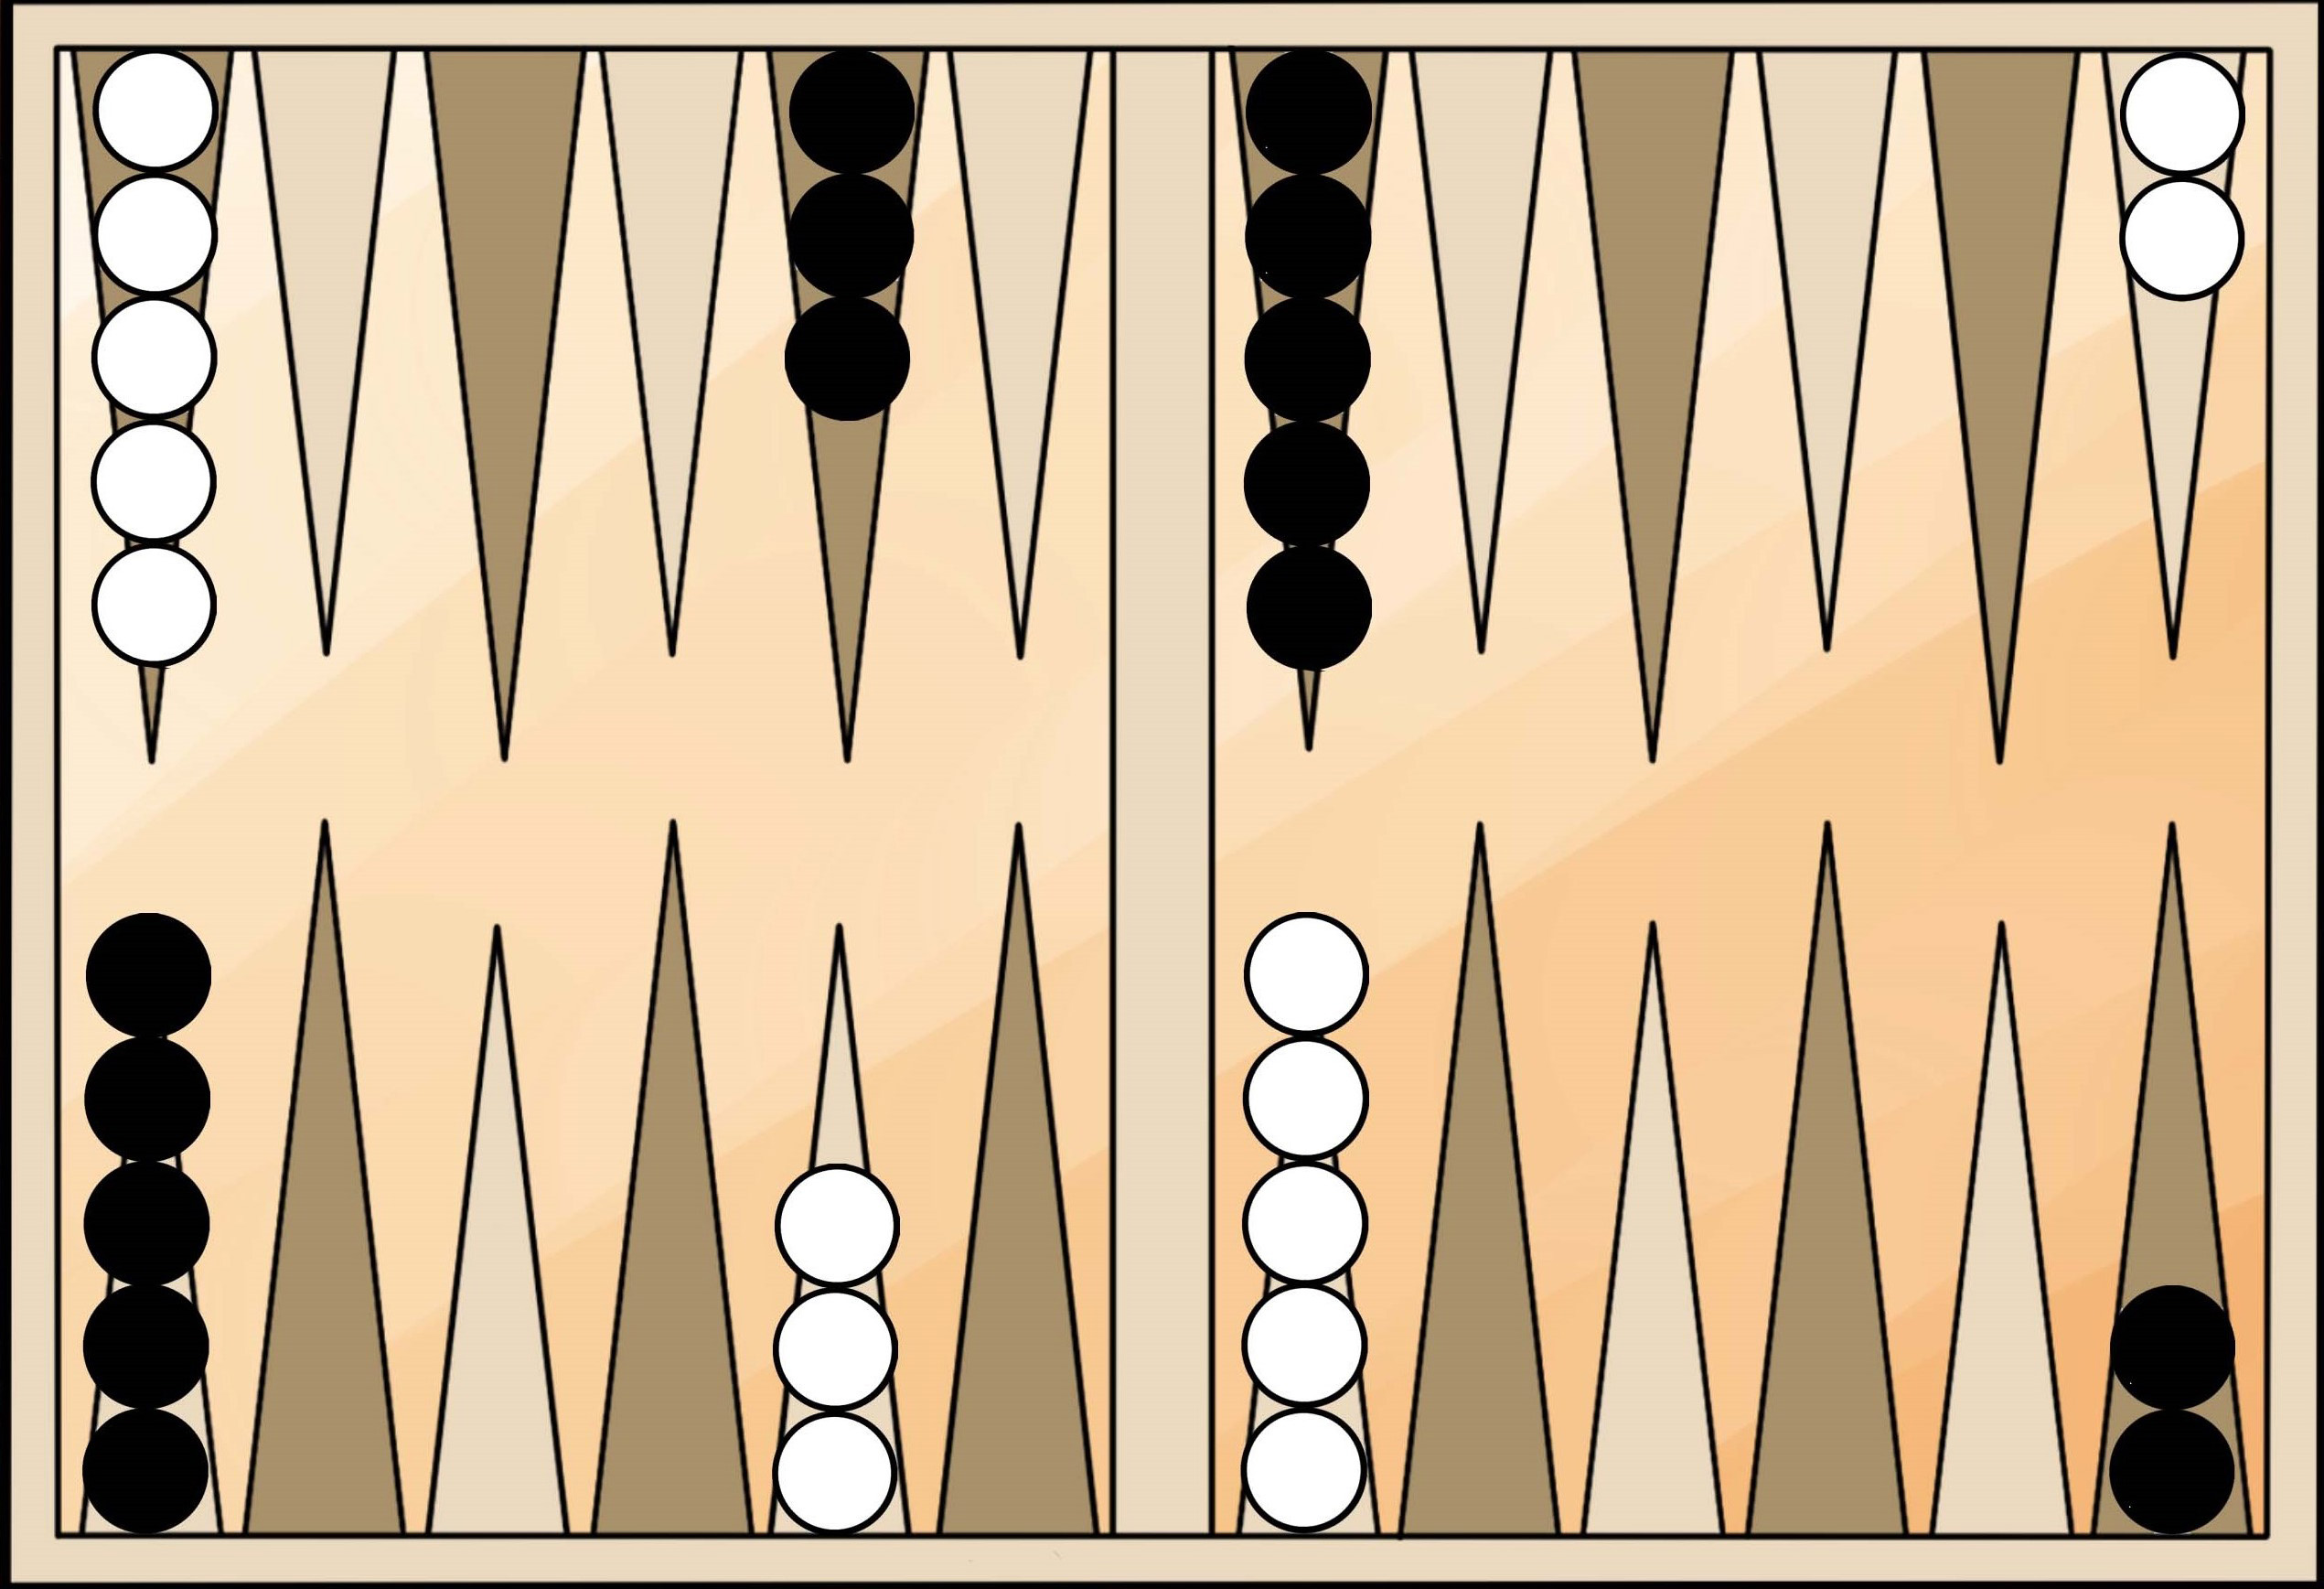
\includegraphics[width=1\textwidth]{gfx/Backgammon-setup.jpg}
    \caption{Backgammon board setup}
    \label{fig:backgammon_board_setup}
\end{figure}

\section{User Interface}
The user interface is written primarily using React, and ofcause some JavaScript, html and css is used as well. When a player first enters the page they are met with the home page, where they can choose to either register or login. Once a player has registered their information is send to the server where it is stored in a database. Once a player logs in their credentials are checked against the database and if they are correct the player is redirected to a lobby where they can either get matched with another player, more on player matching in the networking section, or go to a statistics page. Note that even though the statistics page is mentioned, and the pages does exist the functionality is not implemented. The statistics page would be a page where a player can see how many games they have won, lost, their win rate, if time had permitted it, it would have been possible to see the statistics of other players as well, along with a score board. There is some security concerns with this, as we will cover in the security section, but as it is not implement neither is the security measures. 

When two players are matched by the server with oneanother the game begins. Once the players are matched they are connected to each other using PeerJS and the game begins.
The game is played on a standard backgammon board with 24 points, 12 on each side. The whole user interface is designed to be intuitive and user-friendly. Everything the user will see is relatively simple in the design, partly because the game itself is rather simple, but also because we wanted to keep the design simple and clean. 

The game board is implemented using the GameBoard component which uses various components to display the pieces and handle user interactions. The styling for the user interface is managed using CSS and images, the images are used to display the pieces and the board, thus we as developers do not have to worry about the styling of the pieces and the board, as it is handled by the images.  

\section{Networking}
There are two types of networking used in this project, the first is the server that the players has to connect to in order to get matched with another player, this happens automatically when a player logs in to the home page of the game. Once the player has logged the server til be aware of the player and will later match the player with another player. The server is a rather simple as it does not have much work to do, it primary role is handle user authentication and then match players. The server is written in C\# and uses ASP.NET as the framework for setting up the server. At the moment the server is running as localhost and is not visible to any devises outside the local network, if we were to launch this program as a real world application it would of cause be hosted on a server appropriate for the task. The second connection is the peer-to-peer connected established between two players once they are connected by the server. As briefly mentioned in the general architecture section, once the connection between the two players are established they disconnects from the server, as it is no longer needed. 
Given that we want to use the server as little as possible, the statistics of the players are stored in the browser, as we will cover in section \ref{sec:security} this poses a minor security risk. There is also the possibility of a player clearing their browser cache and thus losing their statistics, this problem could be solved in many ways, one way could be to store the statistics in a central database much like the users information is sotred in one, we would however perfer to use the server as little as possible, so this is not really an option for us. Another probability is using a peer-to-peer database, thus ensuring that we continue using a mainly peer-to-peer distributed system. It would even be possible to use a blockchain to store the statistics, it might be a bit overkill for our purpose, but it is a possibility. As mentioned earlier we simply store the statistics in the browser, and thus none of the mentioned solutions are implemented, we are however aware of the problem and have thought about possible solutions.

\section{Player Matching}
We have talked some about the matching of players, but not exactly how it works. The goal of the player matching is for the match to be as fair as possible, it would be no fun for either of the players to get matched with one from a different leage. The players are put into one of 6 ggroupes based on the number of wins and if possible the players are matched with someone from their own group. However when there are few players, or even many, it might be the case that there is two player from two different groups where they are the player in that group, in such a case we match those players even though the game might no be fair for the player, but  at least they get to play. One way to make the game more fair is to allow the player with the least skill to remove some of his pieces, thus allowing that player a headstart. The amount of pieces to remove has to be determined either by some standard rule or in collaboration with an expert, as we are not qualified.


\section{Moving the pieces}
The positions of the pieces on the board are stored in two arrays. One describes the number of pieces that are currently on the bar, the other array saves the posion of all the pieces on the rest of the board. 
After each move, the validity has to be checked to ensure each player can only make legal moves. 
For this we need to check for:
\begin{itemize}
  \item White can only move clockwise.
  \item Black can only move counter clockwise.
  \item If there are two or more checkers of one color on a position, the other color cannot place its checkers on that field. 
  \item The checkers of one color cannot be moved more than the sum of the two dice the player rolled.
  \item All checkers of one color have to be in the home board before they can be beared off. 
  \item A player can only move his pieces.
  \item Only the player in turn can make a move.
\end{itemize}

\section{Security}
\label{sec:security}
The major security concern in this project is ensuring that it is with high probability not possible for one of the players to cheat by convincing the opponent that the die he threw was different from what it actually was. In many instances like this there is a third party server that ensures that the parties playing the game is not cheating, but in our case where the game is distributed using a peer-to-peer network, we can not use a third party server as then it would not really be a peer-to-peer network. To solve this problem we have designed a cryptographic protocol that with high probability ensures that the players can not cheat. The protocol is as follows: 

For simplicity, we note that the die has 6 sides and that the players are called A and B
\begin{enumerate}
  \item A picks a random number $r_A \in \{1,2,3,4,5,6\}$ and a nonce $n_A \in \{0,1,\dots 2^{128}-1\}$
  \item A uses a cryptographic hash function $H$ to calculate $h_A = H(r_A || n_A)$ where $||$ denotes concatenation
  \item B picks a random number $r_B \in \{1,2,3,4,5,6\}$ and a nonce $n_B \in \{0,1,\dots 2^{128}-1\}$
  \item B uses a cryptographic hash function $H$ to calculate $h_B = H(r_B || n_B)$ where $||$ denotes concatenation 
  \item A sends $h_A$ to B
  \item B sends $h_B$ to A
  \item Once A has received $h_B$ and B has received $h_A$ they send $r_A, \; n_A$ and $r_B, \; n_B$ respectively to the other player.
  \item The players check if $H(r_A || n_A) = h_A$ and $H(r_B || n_B) = h_B$ if this is the case a fair die has been thrown and the protocol continues. If not cheating is suspected and the game is terminated.
  \item Both players compute the value of the die as $(r_A + r_B \mod 6) + 1$
\end{enumerate}
The protocol is designed to mimic a fair die, each player contributes with a random number for the die, as the number is random the opponent has no way of knowing what number is picked and thus has no way of influencing the outcome of the die. The nonce is used such that the opponent can not reuse or brute force the hash function to find the number that the opponent picked.

There is a small caveat to the protocol, if a player is able to brute force the hash function, he can cheat. This is however not really a problem as we are using a cryptographic hash function, which there is no efficient way of brute forcing, furthermore the protocol uses a nonce of 128 bits and a one bit number, which means that there is $2^{129}$ possible combinations for each die throw, which is infeasible to brute force. If further security is needed the nonce can simply be increased to a larger number, or slow hashing can be used.

A second security problem that is worth the at least have thought about is the possibility of a player to manipulate the number of games won. It is a problem that we have not taken security measures against, the main reason is that if a player is able to manipulate the number of games won, the player is really only cheating themselves. Given that players are matched based on the number of games won, the player will be matched with players that are better than them, and thus the cheating player will properly just lose the game. Furthermore, there is currently no way to profit monetarily from this game. Now that we have covered that there is no incentive to falsely increase the number of games won, a player might be lower the number of games won to get matched with players that are worse than them, this is not a new problem as a player can simply make a new account and get matched with players on the same level as the new account. This is a problem that is inherent to all games that are based on the number of games won, and is not something that we have taken measures against.

%% Stealing the cookies of another player
We have covered how a player might be able to manipulate their own score, but not if they can manipulate the score of other players. Given that the player statistics is currently stored in the browser as a cookie, it might be possible for an adversary to steal the cookie and thus manipulate the score of the player. The attack is quite cumbersome and requires more knowlage than the average backgammon player has, we have not taken measures against this possible attack, as it beyond the scope of this project. The problem can however be avoided by encrypting the cookie using a player specific key, though this introduces a new array of problems such as key management and key distribution. Another possibility is just storing the statistics in some other manner, such solutions have been mentioned, but again it is not something that we have implemented.


\section{Implementation}
Our project uses multiple programming languages and technologies to implement that game and server connection to connect the players. The server part is written primary in C\# and uses ASP.NET as the framework for setting up the server. The game itself is written in JavaScript and primarily uses the React library for the user interface.

Below is a list of how the project is structured and what the most central files and folder are.
\begin{itemize}
  \item \textbf{react-client/scr}
  \begin{itemize}
    \item \textbf{components:} Contains all the components that is used on the client side of the game. Each component is responsible for a specific part of the game, the \textit{GameBoard.js} component is responsible for rendering the board and handling the game logic. \textit{SignIn.js} and \textit{SignUp.js} are responsible for handling the user authentication. The components like the name suggests are individual components that is responsible for a specific part of the game. 
    \item \textbf{pages:} The pages folder contains the different pages that is used in the program, such as the home page, the lobby and game page. Where the components are responsible for a specific part of the game, the pages are responsible for the pages that the components are rendered on.
    \item \textbf{routes:} The routes folder contains the different routes that the user can take in the game, such as the home page, the lobby and the game page. The routes are responsible for ensureing that the user is redirected to the correct page when an action is taken.
  \end{itemize}
  \item \textbf{asp.net-server/ASP-Server:}
  \begin{itemize}
    \item \textbf{Controllers:}
    \item \textbf{Models:}
    \item \textbf{Services:}
    \end{itemize}
\end{itemize}



\subsection{Backlog}
The following is a list of features that we would have liked to implement, but did not have time to implement. Some of the features are not essential to the game, but would have been nice to have. The features are listed in no particular order.
\begin{itemize}
  \item \textbf{Statistics:} A page where the player can see their statistics, such as number of games won, number of games lost, win rate etc.
  \item \textbf{Distributed Database:} As mentioned in the networking section, the statistics are stored in the browser, this poses a security risk, and it would have been nice to have a distributed database to store the statistics.
  \item \textbf{Double Dice:} When a player throws a double, the player can move four times the value of the die, this is not implemented in the game.
  \item \textbf{Crawford rule:} The Crawford rule states that if a player is one point away from winning the game, the opponent can not double the game. 
  \item \textbf{Handicap:} If a player has a higher win rate than the opponent, the opponent can remove a number of pieces from the board before the game begins.
\end{itemize}




\chapter{Evaluation \& Conclusion}
\label{cha:evaluation}

\section{Tests}
Due to the high level of interactive and graphical nature of this project and backgammon itself, most of the testing has been done manually, both because a test does not really tell if a design is pretty or intuitive, and because the manual testing helpes us understand how the system behave. While automated testing is definitely useful have focused on manual tests. 

\section{Cost of Distribution}
Given that we have chosen to use a peer-to-peer network where the peers are equal, i.e. no peer has more influence than the other, it means that one can not nessesarily trust the other peer. As we have seen in the security section, there is a need for a cryptographic protocol to ensure that a player can not gain an advantage by influencing the outcome of the die. The protocol designed is quite simple and does not require much computational power, but it does require the players to send some informatio to eachother. Lets take a look at the protocol, and see how much information is send between the players. A player has to send both the number chosen, a nonce and the hash value of the concatenation of the number and nonce. The number is a number between 1 and 6, the nonce is a 128 bit number and the hash value is a 256 bit number, thus the total amount of information send between the players is $1bit+128bits+256bits = 385bits$, for each die throw, for each turn two throws are made, thus the total amount of information send between the players is $385bits*2 = 770bits$ per turn. This is by no means a lot of information. It is however only for one turn, lets assume that each player has 15 turns, thus a total of $15*2*2 = 60$ dies has to be thrown, thus the total amount of information send between the players for an entire game is $770bits*60 = 46200bits = 5.775kB$. Just for the dies. Now lets look at the state of the board, a move in backgammon is denoted as $4-2:\; 10/6\; 8/6$ where $4-2$ denotes that a four and two was thrown, $10/6$ denotes that a piece was moved from position 10 to 6 and $8/6$ denotes that a piece was moved from position 8 to 6. Such a message can be encoded as 10 bits, thus the total amount of information send between the players for an entire game is $10bits*15*2 = 300bits = 37.5B$. Thus the total amount of information send between the players for an entire game is $5.775kB + 37.5B = 5.8125kB$. This is by no means a lot of information, and the cost of distribution is quite low. 

If we were to have implemented the die throw and the board state in a trusted third party, the amount of information that had to be send between the players would be significantly lower, there would be no need for hashes or nonces, the only information that had to be send between the players would be the board state and the die throw. The die throw is a single bit,, where the board state is 8 bits, given that the server knows the dies values. The 8 bits first is sent from the player that made the move to the third party and then from the third party to the other player. The amount of information for the dies is thus $15*2*2 = 60bits = 7.5B$ and the amount of information for the board state is $15*2*8*2 = 480bits = 60B$, thus the total amount of information send between the players for an entire game is $7.5B + 60B = 67.5B$. This is significantly lower than the amount of information send between the players in a peer-to-peer network. This would though require a trusted third party, which is not desirable in a peer-to-peer network.


\appendix
\cleardoublepage

\chapter{An appendix}
\label{cha:an-appendix}

\section{GitLab Repository}
The code for the project can be found at the following GitLab repository. Note that at the time of writing the repository is private and thus requires access to view. It is however expected that the repository will be made public at some point in the future.\\
\gitlab{https://gitlab.au.dk/au702308/building-the-iot}

\section{YouTube demonstration video}
A demonstration video of the project can be found at the following YouTube link.\\
\youtube{Link to YouTube video}



%%%%%%%%%%%%%%%%%%%%%%%%%%%%%%%%%%%%%%%%%%%%%%%%%%%%%
%%%              Stop editing here                %%%
%%%%%%%%%%%%%%%%%%%%%%%%%%%%%%%%%%%%%%%%%%%%%%%%%%%%%

%********************************************************************
% Other Stuff in the Back
%*******************************************************
\cleardoublepage%********************************************************************
% Bibliography
%*******************************************************
% work-around to have small caps also here in the headline
\manualmark
\markboth{\spacedlowsmallcaps{\bibname}}{\spacedlowsmallcaps{\bibname}} % work-around to have small caps also
%\phantomsection 
\refstepcounter{dummy}
\addtocontents{toc}{\protect\vspace{\beforebibskip}} % to have the bib a bit from the rest in the toc
\addcontentsline{toc}{chapter}{\tocEntry{\bibname}}
\label{app:bibliography}
\printbibliography


% ********************************************************************
% Game Over: Restore, Restart, or Quit?
%*******************************************************
\end{document}
% ********************************************************************

%%% Local Variables:
%%% mode: latex
%%% TeX-master: t
%%% End:
